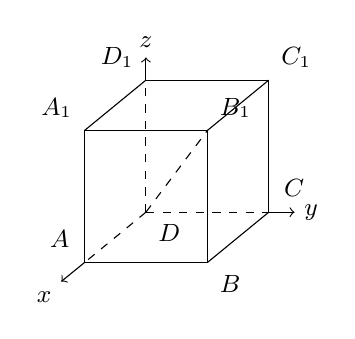
\begin{tikzpicture}[x=0.78cm,y=0.78cm,every node/.style={font=\small}]
  % Source-faithful cuboid topology; projection lengths are schematic.
  \coordinate (D)  at (0,0);
  \coordinate (A)  at (-1.0,-0.82);
  \coordinate (C)  at (2.0,0);
  \coordinate (B)  at (1.0,-0.82);
  \coordinate (D1) at (0,2.15);
  \coordinate (A1) at (-1.0,1.33);
  \coordinate (C1) at (2.0,2.15);
  \coordinate (B1) at (1.0,1.33);

  % Visible cuboid edges.
  \draw (A) -- (B);
  \draw (B) -- (C);
  \draw (A) -- (A1);
  \draw (B) -- (B1);
  \draw (C) -- (C1);
  \draw (A1) -- (B1);
  \draw (B1) -- (C1);
  \draw (C1) -- (D1);
  \draw (D1) -- (A1);

  % Hidden cuboid edges along the three coordinate axes.
  \draw[dashed] (D) -- (A);
  \draw[dashed] (D) -- (C);
  \draw[dashed] (D) -- (D1);

  % The source also shows the vector DB_1 as a dashed diagonal.
  \draw[dashed] (D) -- (B1);

  % Positive coordinate directions continue beyond the corresponding vertices.
  \draw[->] (A) -- (-1.38,-1.13) node[below left] {$x$};
  \draw[->] (C) -- (2.42,0) node[right] {$y$};
  \draw[->] (D1) -- (0,2.52) node[above] {$z$};

  \node[below right=1pt] at (D) {$D$};
  \node[above left=2pt] at (A) {$A$};
  \node[below right=1pt] at (B) {$B$};
  \node[above right=2pt] at (C) {$C$};
  \node[above left=1pt] at (D1) {$D_1$};
  \node[above left=1pt] at (A1) {$A_1$};
  \node[above right=1pt] at (B1) {$B_1$};
  \node[above right=1pt] at (C1) {$C_1$};
\end{tikzpicture}
